\documentclass[conference]{IEEEtran}
% \IEEEoverridecommandlockouts
% The preceding line is only needed to identify funding in the first footnote. If that is unneeded, please comment it out.
\usepackage{cite}
\usepackage{float}
\usepackage{amsmath,amssymb,amsfonts}
\usepackage{algorithmic}
\usepackage{graphicx}
\graphicspath{{./images/}}
\usepackage{textcomp}
\usepackage{subfig}
\usepackage{xcolor}
\def\BibTeX{{\rm B\kern-.05em{\sc i\kern-.025em b}\kern-.08em
    T\kern-.1667em\lower.7ex\hbox{E}\kern-.125emX}}
\begin{document}

\title{Investigating the Effect of Dataset Representivity for Image Colourisation}

\author{\IEEEauthorblockN{Andrew Boyley}
\IEEEauthorblockA{\textit{School of Computer Science} \\
\textit{and Applied Mathematics}\\
\textit{University of the Witwatersrand}\\
Johannesburg, South Africa \\
andrew.boyley@students.wits.ac.za}
\and
\IEEEauthorblockN{William Hill} 
\IEEEauthorblockA{\textit{School of Computer Science} \\
\textit{and Applied Mathematics}\\
\textit{University of the Witwatersrand}\\
Johannesburg, South Africa \\
william.hill1@students.wits.ac.za}
\and
\IEEEauthorblockN{Steven James}
\IEEEauthorblockA{\textit{School of Computer Science} \\
\textit{and Applied Mathematics}\\
\textit{University of the Witwatersrand}\\
Johannesburg, South Africa \\
steven.james@wits.ac.za}
}

\maketitle

\begin{abstract}

Sufficient research exists for the implementation of bias-mitigating machine learning algorithms, however, the presence of bias in the original dataset has not been comprehensively considered, which could lead to vast improvements in the efficiency and diversity of machine learning in general. To determine what percentage of local data has to be included in order to alleviate this bias, we examine the sub-problem of how much South African data is required to correctly colourise grayscale images of a South African context. There was only a 3.3\% reduction in the error of the colourised images using separate regression-based models trained to 75 epochs with 0\% to 30\% inclusion of local data, with minimal reduction in loss occurring after 5 epochs. This did lead to the hues of the images being slightly more South African in essence, but which was largely unnoticed by the human eye. Consequently, the inclusion of local data in the dataset definitely minimises the bias of the dataset, but whether or not that bias-mitigation justifies the vast resources required to build the comprehensive dataset is determined on a case-by-case basis.

\end{abstract}

\begin{IEEEkeywords}
deep learning, bias, dataset imbalance, regression, self-supervised learning, image colourisation
\end{IEEEkeywords}

\section{Introduction}

Machine Learning is a tentative endeavour, whereby subtle changes in the learning environment often lead to profound alterations to both the overall effectiveness of the machine learning model and the accuracy of the desired output. 

Such a phenomenon exists when training a model to recognise and colourise aspects of grayscale images: by employing a training dataset with a bias to a particular locale – like an American or a Eurocentric setting, for instance – any sample taken from outside such an area (with particular focus placed on a South African sample) is misrepresented and yields erroneous results, with the produced colourised image being quintessentially different to the intended image.

The identified cause is the lack of diversity in the training datasets because even though various methods can be implemented in the actual model to mitigate this bias, they cannot account for a wholly prejudiced dataset being used initially, particularly a non-South African dataset being used to train a model to operate on a South African sample. 

Therefore, the aim is to investigate what percentage of the training dataset has to be of local origin compared to the international origin of the remainder of the dataset. However, constructing and testing datasets to determine such a goal is both time consuming and expensive in terms of financial and computational resources required. Hence, the approach of image colourisation has been selected as it allows an uncomplicated procedure of collecting publicly-available images of both International and South African settings, thus providing a simple way to build a diverse dataset which does not need to be labelled or require excessive computational time since the machine learning approach required is one of supervised learning where the expected outcome is derived from the images themselves.

Consequently, the refined aim is to investigate the optimal ratio of non-South African images to South African images in the training dataset is such that bias is minimised and the model performs optimally for both sets of images.

\section{Background}

\subsection{Colour space}

For simlicity, rather than using the typical RGB colour space, we make use of the CIELAB colour space. This makes it convenient when seperating the gray and colour channels due to the fact that the 'L' channel in LAB is simply the grayscale image. This grayscale input (1 x W x H) is then passed through the model and compared with the output (2 x W x H) of the original 'AB' channels of the image. These 'AB' channels make up the colour and simply signify the red-green and blue-yellow shift respectively. HSB would be another option when choosing a suitable colour space. In general, the choice of colour space makes no difference to the resulting image that our network produces.

When reading images from our dataset, our chosen system interprets them in the RBG colour space and then proceeds to convert them to LAB using tools such as SciKit Learn or OpenCV, both of which contain colour space conversion libraries. 

\subsection{Regression vs Classification}

When colorizing images using a deep learning approach, it is generally easiest to develop the model as a regression problem. Classification would yield better results which are more life-like and saturated whereas regression would lead to output images appearing dull and bland. This is the result of the multi-modality of pictures. There is no clear colour for any one image. This leads our model, using an aggregate loss function, to simply find an average colour, resulting in a bland image.

\begin{figure}[h]
    \centering
    \subfloat[Regression]{{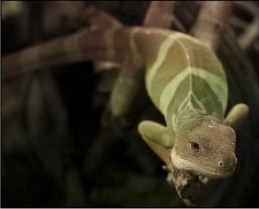
\includegraphics[width=3.5cm]{cham-reg} }}%
    \qquad
    \subfloat[Classification]{{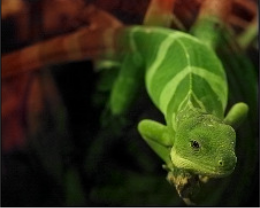
\includegraphics[width=3.5cm]{cham-class} }}%
    \caption{Colour generated using regression vs classification \cite{zhang2016colorful}}%
    \label{fig:reg_vs_class}
\end{figure}

For the sake of simplicity, we continue to use regression as it leads to satisfactory results whilst being simple to understand. We utilize a mean squared error loss which may average colour distribution but still produces images with a reasonable amount of colour. If we aimed to produce images which were more diverse in colour and saturated, regression would not suffice. Our model should, however, be able to compare output across datasets in order to draw correlation between the accuracy of the ouput and the representivity of local images in the data, which it does.

\subsection{Model topology}

Our choice of model has been based on the simple regression model developed by Luke Melas \cite{melas2018mark} and loosely based on the network used by Zhang et al. \cite{zhang2016colorful}\cite{zhang2017real} with the major difference being that their model used in 'Colorful Image Colorization'\cite{zhang2016colorful} approached colourisation as a classification problem.

Our network topology consists of the first six layers of a ResNet-18, followed by three layers of deconvolutions. We find that this simple structure works well enough for our purposes and is relatively fast. Our model uses the Adam optimiser alongside PyTorch's autograd which makes backpropogating in our network trivial.

\section{Proposed Method}


\subsection{Brief Outline}

In order to determine the percentage of local data in the training dataset required to mitigate the effect of bias in machine learning models, multiple versions of the dataset are required, with each one consisting of a total of 40000 images and being constructed with a different percentage of South African images from 0\% to 30\% inclusive, increasing in graduations of 10\%. In addition to this training dataset, a validation dataset (of 1000 images in total) is also prepared with the same corresponding percentage inclusion of South African images.

Each version of the dataset will be used to train the model independently of each other for a total of 75 epochs each, with validation being done at the conclusion of each epoch. 

A set collection of South African and International images will be passed through each model respectively, with the subsequent losses being an indication of the bias present in the model due to the predominant locale present in the training images (we take the dataset version with 0\% South African images included as the base case of how the model performs on South African image evaluation when trained exclusively on International images).

\subsection{Building Datasets}

Our original dataset is a subset of the Places365 dataset. This dataset consists of images that are mainly of European or Western origin. This means that if we train a model on such a dataset and then prodceed to evaluate it on South African or local images, we expect an increase in our loss. This drop in performance can be attributed to the difference in colour of local images. For example, South African landscapes have a distinct hue that is not present in European countries. South African people also have a different appearance to western people who will likely be present in European datasets.

The collection of South African images\footnote{All images are freely available with a Creative Commons Licence or are in the public domain} was downloaded from the image-sharing service, Flickr. Only images which have been tagged with one of the following keywords were selected:

\begin{itemize}
	\item South Africa
	\item Soweto
	\item Johannesburg
	\item Kruger Park
	\item etc.
\end{itemize}

A Python script was used to assimilate the International and South African images into the required ratios (of 0\% to 30\% South African image inclusion) by randomly sampling $x$\% of images from the South African training split and $x$\% of images from the South African validation/testing split. The same number of images ($x$\%) was removed from the foreign dataset meaning that for each dataset, it contains $x$\% local data and ($100 - x$)\% foreign data where $x\in\{0, 10, 20, 30, 40\}$

\begin{table}[h!]
\centering
\begin{tabular}{cc}
\includegraphics[width=3.7cm]{SampleSA/46} & 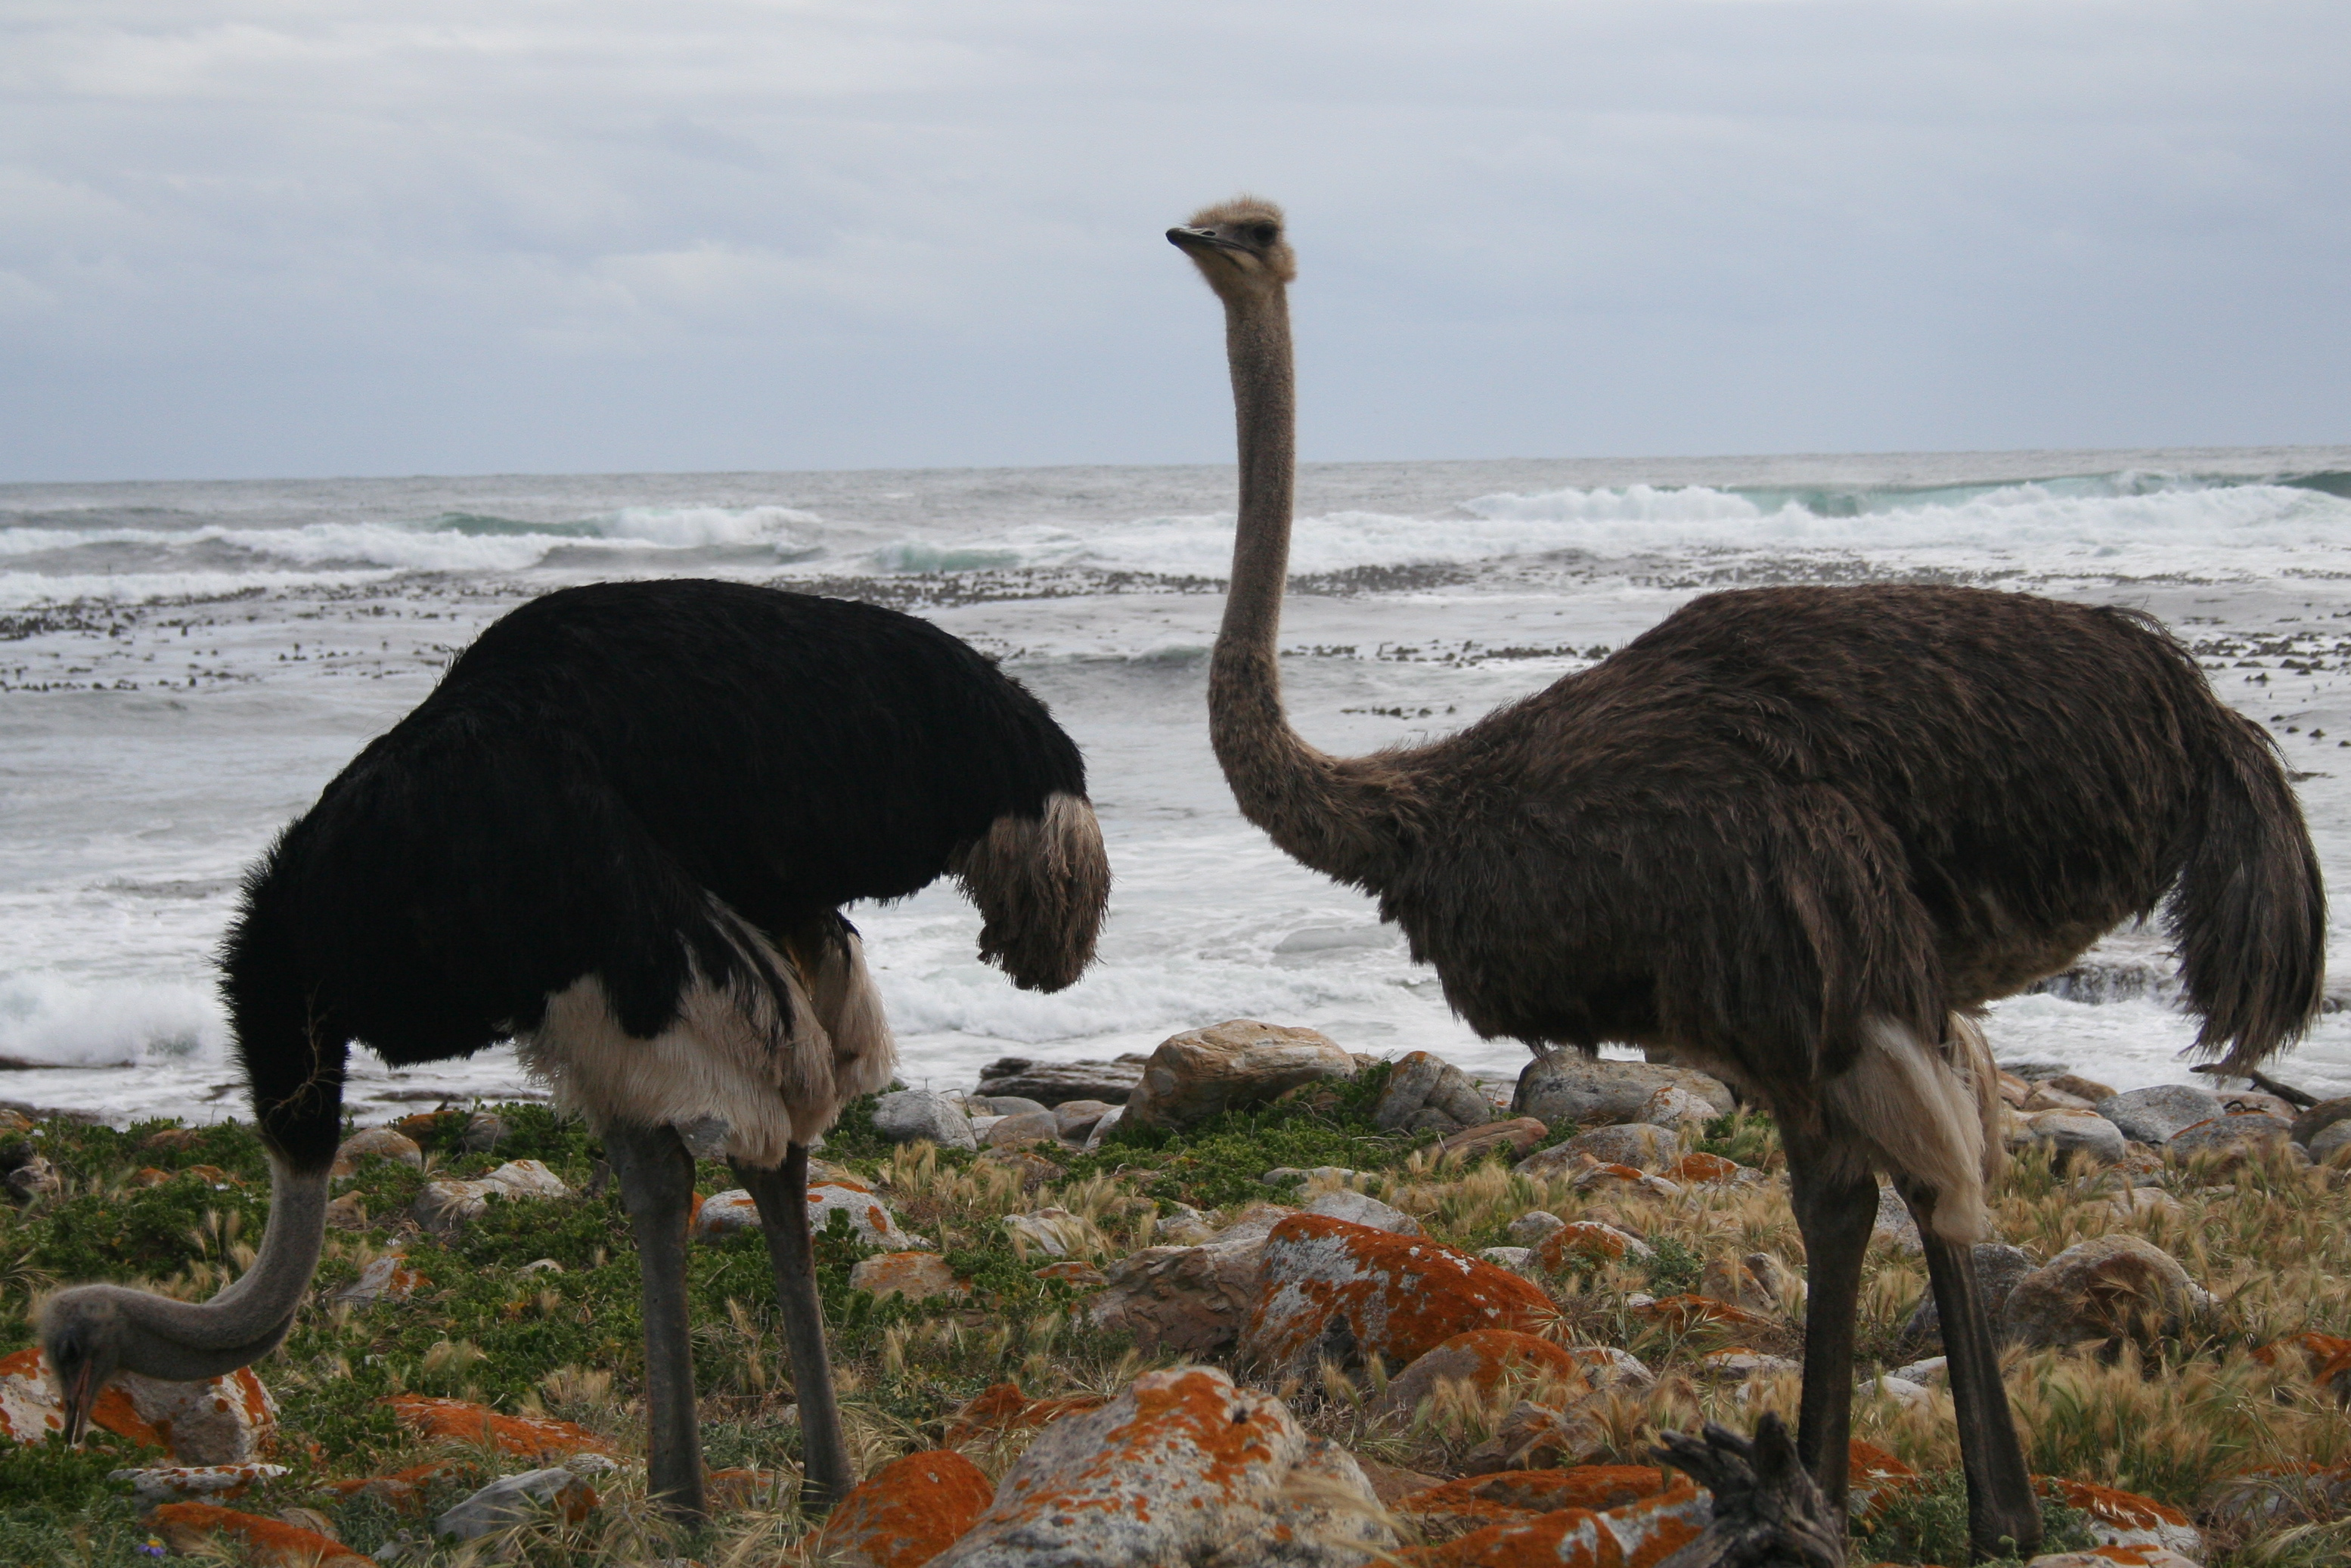
\includegraphics[width=3.7cm]{SampleSA/61}\\
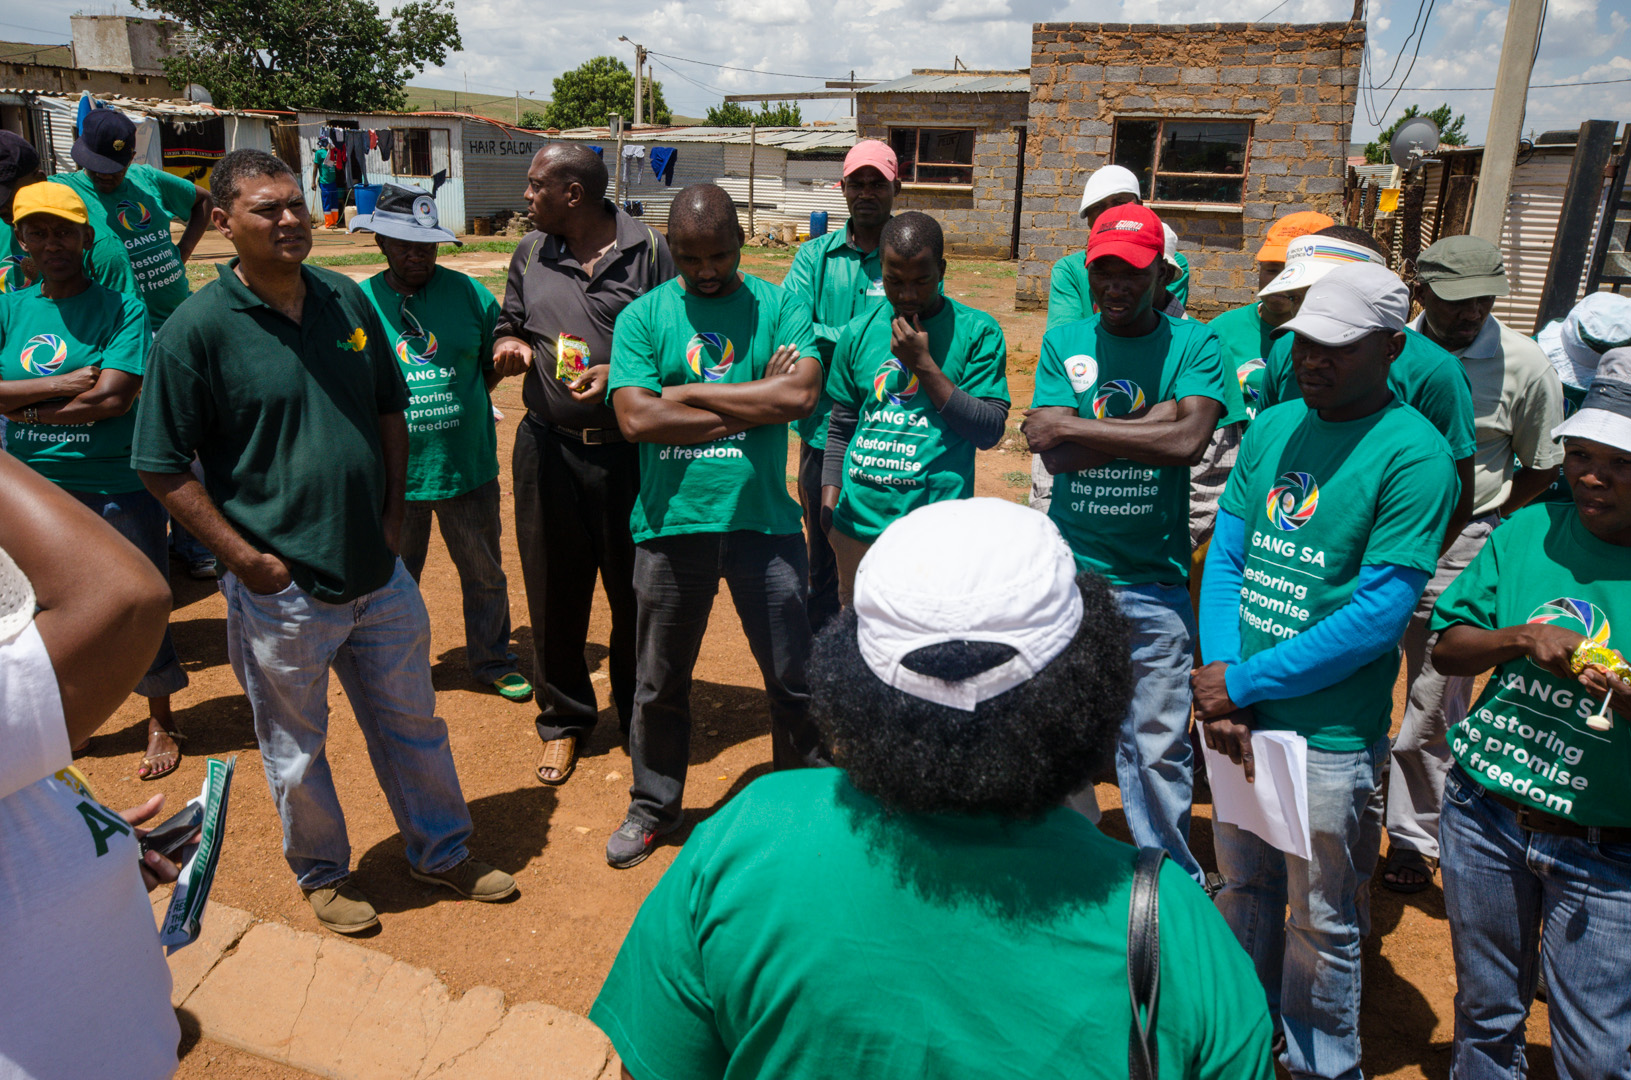
\includegraphics[width=3.7cm]{SampleSA/106} & 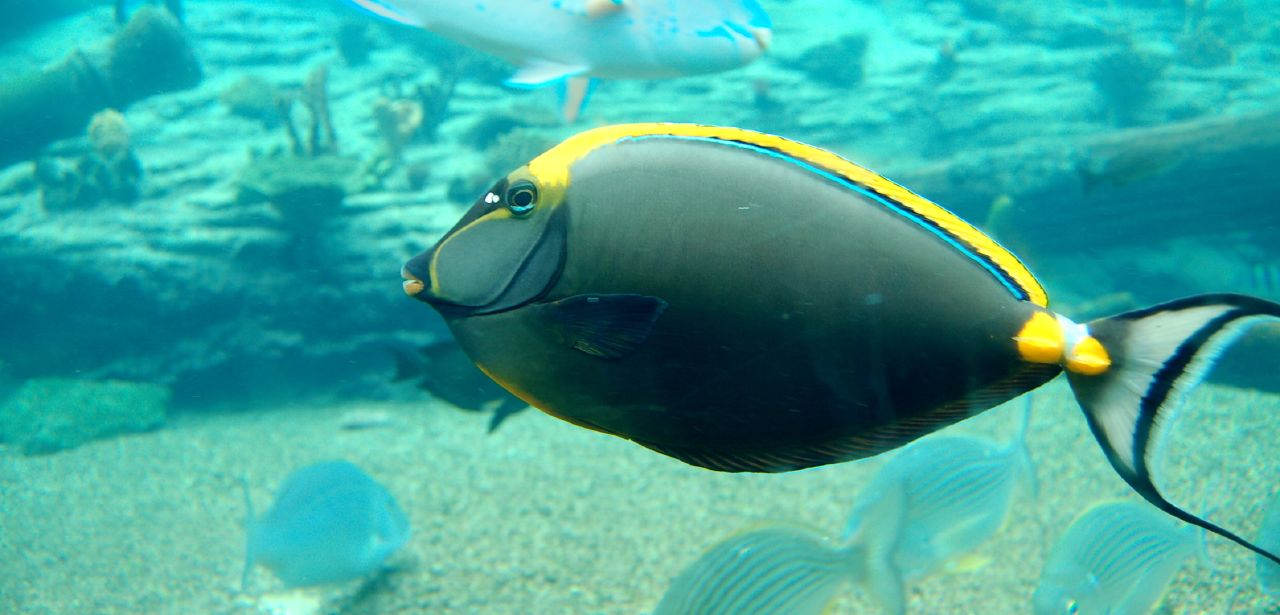
\includegraphics[width=3.7cm]{SampleSA/127}\\

\end{tabular}
\caption{Sample images from the South African dataset}
\label{fig:samplesa}
\end{table}

\section{Experiments}

%Explain experiment. Model used. Hyperparameters. Early stopping?? Train/val/test splits.
%
%Show training curves over time for model trained on X. 
%
%Show images from X coloured.
%Show images from Y coloured - qualitative analysis
%
%Start adding data from Y to X. 
%
%Produce THE curve as a function of data ratio
%
%Show images from X coloured.
%Show images from Y coloured - qualitative analysis

\subsection{Training}

For each dataset, we trained our convolutional model from the beginning with the exact same hyperparameters. The following table illustrates the hyperparameters used:


\begin{table}[h]
\centering
\renewcommand{\arraystretch}{1.5}
\begin{tabular}{|c|c|c|c|}
\hline 
Learning Rate & Epochs & Workers & Batch Size \\ 
\hline 
0.001 & 75 & 4 & 64 \\ 
\hline 
\end{tabular} 
\end{table}

Due to the fact that images collected from Flickr were substantially larger in size than those of the European set, it took longer to train models with a high inclusion rate to the above mentioned epoch. For this reason, we chose to limit our inclusion of South African data to 30\%. Future experiments could show that an inclusion rate higher than 30\% is optimal but for the purpose of this experiment, it will suffice.

For the sake of simplicity, validation and test sets have been merged into one. For each dataset, there are 40000 images in the training set and 1000 in the test/validation split. This makes it an average sized data set which means that the inclusion rates on these datasets shoud reflect to other datasets of similar size with only minor deviation.

\begin{figure}[h]
\centering
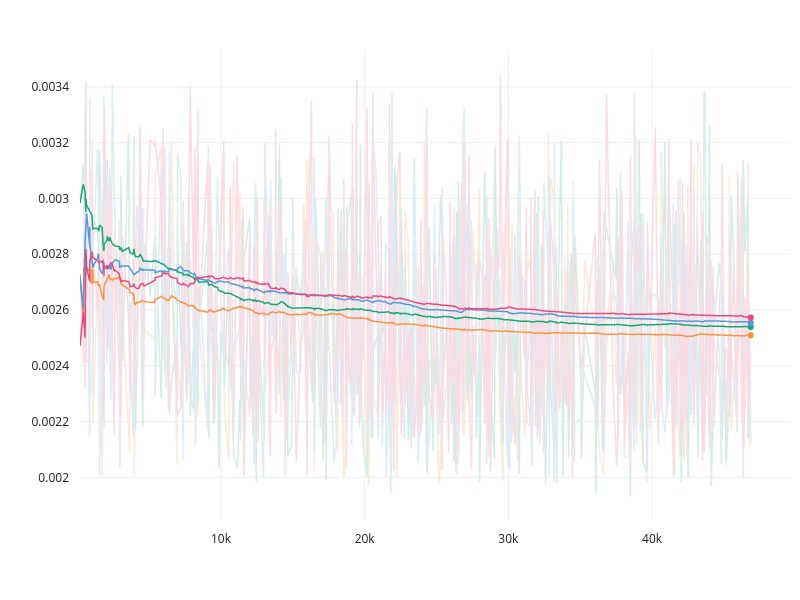
\includegraphics[width=9cm]{Curves/loss_train}
\caption{Loss curves of each dataset during training}
\label{fig:loss_train}
\end{figure}

We found that the loss dropped immediately to a reasonable value within the first five epochs but the images produces were not of a high quality. The training process was long and slow with very little change in loss from one epoch to the next but the end results make it worthwhile. Better results could have been achieved by training more models, each with a different inclusion of local data. This would allow us to draw a definative correlation of local data to loss but in this case, the samples we have taken will give us a very rough idea of the optimal parameters.

%Insert picures from different epochs

\subsection{Evaluating}

After all models have been trained on their respective datasets, we evaluate them on purely the South African dataset. This gives us a good understanding of how much local data to include into foreign datasets if we want reasonable results. The pure South African dataset contains 35000 images in its training split and 5000 images in the validation/testing split. These were both used to construct the hybrid datasets. Now, we evaluate the model that has been previously trained on the foreign-local hybrid set on a purely South African dataset and measure its performance.

We expect the loss to be much larger when very few South African images have been included into the hybrid set. As we evaluate datasets with a larger inclusion of local data, we expect the models loss to decrease. Using this data, we can estimate the optimal inclusion of local data for satisfactory results when performing machine learning in foreign countries.

After evalutating each model on the same purely South African dataset, these are their respective losses,

\begin{table}[h]
\centering
\renewcommand{\arraystretch}{1.5}
\begin{tabular}{|l||c|c|c|c|}
\hline 
Local inclusion \% & 0\% & 10\% & 20\% & 30\%  \\
\hline
Loss $\times 10^{-3}$& 2.727 & 2.696 & 2.660 & 2.638\\ 
\hline 
\end{tabular} 
\end{table}



As you can see, the diffrence in loss is miniscule. The small drop in loss that you get when including local data is not worth the time and effort spent retrieving, processing and preparing it in the first place. The majority of datasets used in image colourisation or classification already contain a wide variety of images that will make including local data redundant. By no means does this mean that the inclusion of local data plays no role in producing better looking images that more closely resemble the place of origin. It does, however, mean that the inclusion of local data simply does not effect the outcome of the experiment as much as other factors would. Other factors include running the experiment for longer or simply finding a larger dataset. The insignificance of local data inclusion is made extremely evident when comparing images that were produced using a model trained without any local data with a model trained using 30\% local data,

\begin{figure}[h]
    \centering
    \subfloat[0\% inclusion]{{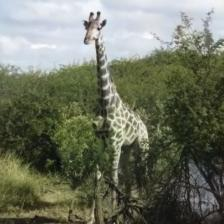
\includegraphics[width=3.8cm]{Inclusion_compare/0} }}%
    \qquad
    \subfloat[30\% inclusion]{{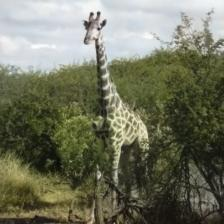
\includegraphics[width=3.8cm]{Inclusion_compare/30} }}%
    \caption{A colourised image produced using models with varying inclusion of local data}%
    \label{fig:inclusion_compare}
\end{figure}

The difference above is extremely minute. You may not even be able to see the difference but upon closer inspection, the image produced with local data contains greens that are more yellow and brighter as well as grass that is more vivid and South African. These changes may very well go unnoticed and coincide with the small changes observed in the loss value.

\section{Related Work}

Many studies have shown that the majority of datasets used in facial analysis are comprised of mostly lighter skinned subjects. Research published by Joy Buolamwini \cite{buolamwini2018gender} shows that when evaluated on industry standard facial analysis networks, dark skinned females yield the highest error rates (of up to 34.7\%). This is alarming considering that light skinned males yield a maximum error rate of only 0.8\% when evaluated on the same dataset. \cite{corbett2018measure}

This stems from the fact that data scientists and researchers continue to neglect the unbalanced distribution of race in the datasets that they use. The systems used and sold by IBM, Microsoft and Amazon are just a few that contain these race imbalances. The systems sold by these technology giants are used by some states in the United States to apprehend criminals by means of facial recognition. The fact that there are racial imbalances in many of the networks used in these systems means that there is a higher chance for people of colour to be falsely accused of criminal activity due to facial recognition software returning a false positive. 

The class imbalance problem has long been researched and there are various methods \cite{japkowicz2000class} to overcome the issue. One such method to overcome a dataset imbalance is to simply re-sample the minority until a suitable distribution is achieved. Similarly, down-sampling the majority leads to a fairer distribution as shown in \cite{japkowicz2000class}. 

No substantial research has been conducted in investigating the effect of data imbalance with respect to image colourisation. This may be due to the fact that image colourisation is largely subjective as made evident in the previous section.

\section{Conclusion}

%Important problem
%
%Investigated data representivity
%
%What we found
%
%Extensions to other tasks.
\subsection{Advantages of Examining Bias}

The investigation of dataset bias on the training of machine learning models is highly relevant as an affirmative conclusion could lead to the development of methods for improving the overall efficiency of the model (as opposed to optimising the actual algorithm used for training) as well as a more thorough representation of the data and the various real-world conditions that exist, thus enhancing the diversity of the application of the model.

\subsection{Interpretation of Colourisation Experiment}

Evidently, the errors in the images coloured for the various percentage inclusions of local data are relatively the same - only a 3.3\% improvement was recorded for the training of the model from the 0\% inclusion to the 30\% inclusion. Such an improvement is mitigated when considering that the error on the colourisation of the images is already of an order of magnitude of $-3$, and is likely only to be noticed by computers and those utilising computational resources to analyse the images.

This slight improvement is evident in the modest variations in the hue of the colours, as in Figure \ref{fig:inclusion_compare}, with the images produced from subsequently-increasing percentages of local data inclusion containing hues and saturations more applicable to that locale.

Consequently, the effect of the inclusion of local data is not as profound as one might have hypothesised and the images produced from a model trained with this local data included are largely indistinguishable from the images produced from a corresponding international dataset, especially to the human eye and so does not justify the additional resources required to build the inclusive dataset.

\subsection{Further Analysis}

Although we investigated the effect of dataset bias on image colourisation, there are a multitude of other applications of machine learning where this bias may come into effect. Due to the inherent differences between the nature of image colourisation and other applications (for example, in examining and predicting economic trends in a particular city), where humans may be abstracted from the analysis of the data and it is does solely by computers with a report merely being generated - in such a case, minute changes are of the utmost importance and lead to significant changes in the market trends recognised.

Therefore, the result of whether or not dataset bias exists is conclusive: it does and the inclusion of more diverse data in the set improves the performance of the model; the result of whether or not the building of a more diverse dataset is inconclusive: this would be decided on a per-application basis and what relative accuracy is required.

\medskip
 
\bibliographystyle{ieeetr}
\bibliography{bibfile}


% \begin{thebibliography}{00}
% \bibitem{b1} G. Eason, B. Noble, and I. N. Sneddon, ``On certain integrals of Lipschitz-Hankel type involving products of Bessel functions,'' Phil. Trans. Roy. Soc. London, vol. A247, pp. 529--551, April 1955.
% \bibitem{b2} J. Clerk Maxwell, A Treatise on Electricity and Magnetism, 3rd ed., vol. 2. Oxford: Clarendon, 1892, pp.68--73.
% \bibitem{b3} I. S. Jacobs and C. P. Bean, ``Fine particles, thin films and exchange anisotropy,'' in Magnetism, vol. III, G. T. Rado and H. Suhl, Eds. New York: Academic, 1963, pp. 271--350.
% \bibitem{b4} K. Elissa, ``Title of paper if known,'' unpublished.
% \bibitem{b5} R. Nicole, ``Title of paper with only first word capitalized,'' J. Name Stand. Abbrev., in press.
% \bibitem{b6} Y. Yorozu, M. Hirano, K. Oka, and Y. Tagawa, ``Electron spectroscopy studies on magneto-optical media and plastic substrate interface,'' IEEE Transl. J. Magn. Japan, vol. 2, pp. 740--741, August 1987 [Digests 9th Annual Conf. Magnetics Japan, p. 301, 1982].
% \bibitem{b7} M. Young, The Technical Writer's Handbook. Mill Valley, CA: University Science, 1989.
% \end{thebibliography}

\end{document}
